\chapter{Gait Generation and Optimization for Modular Robots}
  This chapter will discuss the application of the PDABGA in a gait-optimization
    scenario involving three connected modular robots.
 
\section{Gait Implementation}
  A novel gait control method has been implemented for usage on the Mobot.
  The Mobot has several limitations which prevent the usage of some of the
    high-tech cutting edge gait control laws which have been used for some
    other multi-jointed robots. 
  Specifically, the Mobot can only communicate via Bluetooth and lacks the
    capability of forming Bluetooth piconets. 
  This means that Mobots cannot communicate directly with each other, and
    cooperating Mobots must communicate with a central computational device,
    such as a computer, tablet, or smartphone. 
  Furthermore, the bandwidth of the communication channel is fairly limited.
  These limitations preclude the usage of any gait control method that 
    requires fast communication across modules, such as the majority of 
    distributed gaits and neural nets.

  Therefore, the gait implementation chosen for this research, based on
    previous work done by Yang et. al. \cite{Yang2006}, requires no 
    inter-module communication and very little central control, needing
    only a synchronizing clock from the central controller to function.
  At the same time, the gait implementation is very expressive compared to
    some more primitive gait implementations, such as gait tables.
  It can also theoretically implement any periodic gait, and is easily
    optimizable evolutionary algorithms.
  This is accomplished by representing the motion of each joint of a gait 
    as a list of Fourier series coefficients. 
  The infinite Fourier series, shown in Equation \ref{eq:fourier}, is a
    representation of any periodic function as a summation of sin and 
    cosine functions.

  \begin{equation}
  \label{eq:fourier}
  f(t) = \frac{1}{2} a_0 + 
  \sum_{i=1}^{\infty} a_i \sin\left(\frac{2 \pi i}{T}t\right) + 
  \sum_{i=1}^{\infty} b_i \cos\left(\frac{2 \pi i}{T}t\right)
  \end{equation}
  
  The Mobots used for this research have been augmented with a Fourier series
    control law, shown in Figure \ref{fig:motor_controller_architecture}.
  Basically, the implementation is a Fourier series function generator which
    produces a stream of angle values depending on the current local time and the 
    currently stored Fourier series coefficients.
  The PID controller drives the motor to the best of its ability to follow 
    the signal provided by the Fourier series function generator.
  Note that almost the entire implementation and execution of the Fourier series
    gait happens locally on the robot.
  There are only two extra-modular communication events which need to occur to 
    run a Fourier series based gait.
    \begin{itemize}
      \item First, the central controller needs to modify the stored Fourier series 
        coefficients on each robot. This step is not time critical and may be 
        performed in series over the list of connected robots.
      \item Second, the central controller needs to issue a synchronizition
        signal to all of the robots, acting like a starting gun to start the
        robotic gait. Ideally, this signal should be sent in parallel to each
        robot simultaneously to perfectly synchronize their clocks, but 
        fundamental limitations with Bluetooth prevent this. However,
        the communication events occur on a timescale magnitudes of order
        shorter than robotic motions and thus any delay caused by this step
        are deemed negligable. When each robot receives the synchronization
        signal, it stores it's own current clock time, $t_c$ which is the
        number of milliseconds since the robot has powered on, into a 
        variable $t_s$. The function generator then uses the value
        $(t_c - t_s)$ as the time value in the Fourier series function generator,
        thus synchronizing the function generators across multiple modules.
    \end{itemize}
  
  % FIGURE --------------------------------------------------
  \begin{figure}[!ht]
  \begin{center}
     \includegraphics[width=5in]{figures/motor_controller_architecture}
  \end{center}
  \caption{\label{fig:motor_controller_architecture}Standard Mobot
  motor controller augmented with Fourier series function generator.}
  \end{figure}
  % END FIG -------------------------------------------------

\section{Simulation Design}
  The simulation built in a module fashion to simulate Mobot modules that
    have been attached end-to-end. 
  The composite robots are built in the simulation algorithmically, such that 
    the number of modules simulated can be specified on the command line
    as a command line argument.
  The simulation simulates the basic geometry of the robots using primitive 
    shapes such as boxes and cylinders to detect collisions.
  The ground is simulated as a perfectly flat plane.
  The simulation uses the Open Dynamics Engine (ODE)\cite{ode} as the physics
    engine for detecting collisions, calculating dynamics, and driving the 
    virtual motors.

  The simulation is built for the specific purpose of calculating the fitness
    of a chromosome.
  When a simulation is initialized with a valid chromosome, it simulates a 
    Mobot cluster running a gait based on the chromosome. 
  The simulation simulates the compound robot for ninety seconds of simulated
    time and finds the 2-d euclidian distance the robot has travelled in that
    time, in meters.
  This value in meters is the fitness of the robotic gait. 

  The simulation is built as a completely separate stand-alone application. 
  Using a variety of command line options, it is possible to adjust various
    operating parameters, such as the chromosome and whether or not to render
    graphics.
  It is built as a standalone application such that if it crashes, it does not
    corrupt the memory space of any other applications.
  Another advantage to running the simulations as separate processess is that
    the operating system can divide the simulation instances across multiple
    CPU cores. 
  The agency starts the simulation instances as separate processes and communicates
    with the process using files.

\section{Chromosome Design}
  Each chromosome will contain a number of genes which represents a robotic gait. 
  The chromosome format will be represented as an array of structs, where
  each struct contains the necessary gait information for a single module.
  A naive example struct representation of a chromosome might appear as such:
  \begin{verbatim}
  struct cyclicGait_s {
    float a[N];
    float b[N];
  };

  struct rotationGait_s {
    uint8_t numWaypoints;
    float waypoints[N];
  };

  union faceplateGait_u {
    struct cyclicGait_s cyclicGait;
    struct rotationalGait_s rotationalGait;
  };

  // Chromosome for single Mobot
  struct chromosome_s {
    uint8_t joint1GaitType;
    union faceplateGait_u joint1Gait;
    struct cyclicGait_s joint2Gait;
    struct cyclicGait_s joint3Gait;
    uint8_t joint4GaitType;
    union faceplateGait_u joint4Gait;
  };
  \end{verbatim}

  As shown, the size of each chromosome would be 
  \begin{eqnarray*}
  \mathrm{bytes} &=& M s(\mathrm{chromosome}) \\
  &=& M ( 1 + 2 s(\mathrm{faceplateGait}) + 2 s(\mathrm{cyclicGait}) + 1) \\
  &=& M (2 + 2*2*s(\mathrm{float})*N + 2*2*s(\mathrm{float})*N) \\
  &=& M (2 + 2*2*4*N + 2*2*4*N) \\
  &=& 2M + 32MN
  \end{eqnarray*}
  where $s()$ is the \texttt{sizeof()} function, M is the number of modules, and N is
  the number of terms to evaluate within the Fourier series.
  We can immediately see that the size of the chromosome may be prohibitively large for any reasonable value
  of \texttt{N} and \texttt{M}. For instance, if we choose 10 terms for the Fourier series
  on a 7 module snake, our chromosome size would be an astounding 2254 bytes. However,
  several assumptions and simplifications can be made to reduce the search space. 

  For instance, it may be beneficial to restrict the values of the Fourier coefficients such that 
  they remain within a few orders of magnitude of each other. If the values diverge too much,
  the higher coefficient terms will dominate and the effect of the lower coefficient terms
  may be completely neglected during floating-point addition of the Fourier series. Furthermore, if the output of the function
  $f(t)$ is to be an angle in radians, it may make sense to limit the value of the coefficients
  to some reasonable multiple of $\pm2\pi$, since the body joints may only rotate to values
  of $\pm\pi/2$ anyways. A reasonable criteria is to have enough variability 
  in the coefficients to create a square wave. For a square wave of amplitude $\pi$, the Fourier series coefficients
  are $a_n = 0$ and 
  \begin{equation}
  b_n = \pi \frac{4}{n \pi} [1 - (-1)^n]
  =
  \frac{4}{n} [1 - (-1)^n]
  \end{equation}
  Thus, even if the the coefficients are limited to a value of $8$, it is still possible to
  evolve a square wave type motion that rotates a faceplate joint through its complete range of motion. 
  If we reduce the range and resolution of the coefficients, 
  we may be able to reduce the representation of each one of the coefficients from a 
  4 byte float to a single byte. The byte could be translated to a floating point
  coefficient using pseudocode similar to 
  \begin{verbatim}
  float c = ((unsigned_byte-128)/128) * c_max
  \end{verbatim}
  Furthermore, prior research has shown that even a Fourier series with
  only five elements can produce interesting gait cycles \cite{Yang2006}. 

  % FIGURE --------------------------------------------------
  \begin{figure}[!ht]
  \begin{center}
  \subfigure[N=5] {
     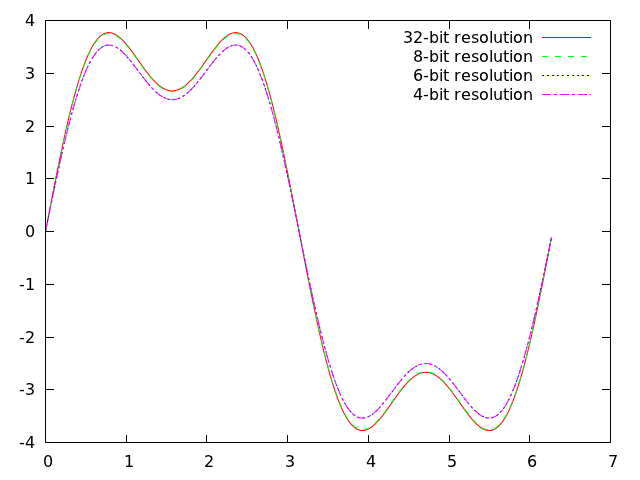
\includegraphics[width=2.5in]{figures/plot_N5}
  }
  \subfigure[N=10] {
     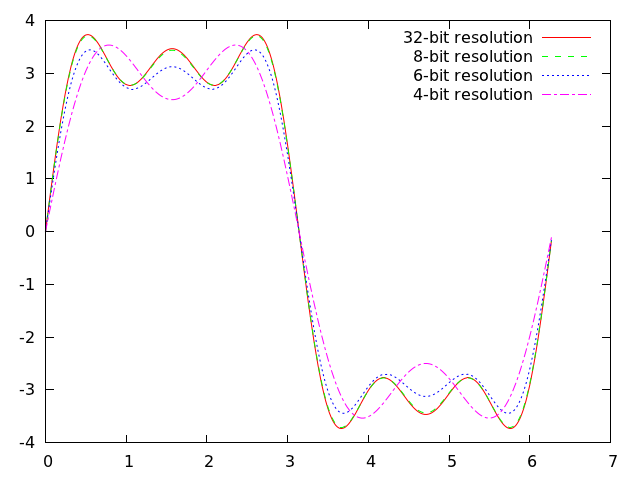
\includegraphics[width=2.5in]{figures/plot_N10}
  }
  \subfigure[N=200] {
     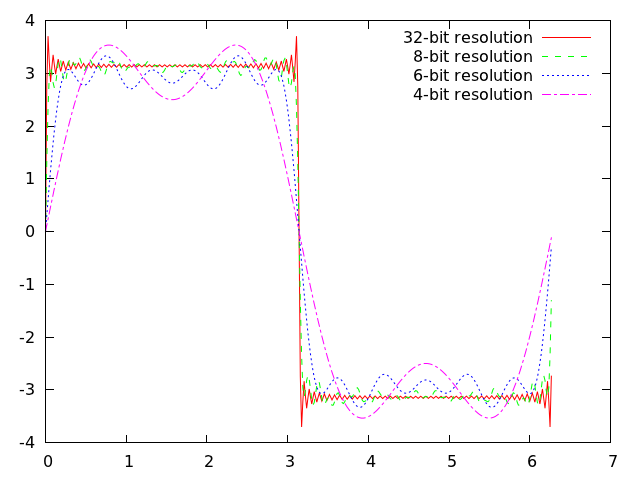
\includegraphics[width=2.5in]{figures/plot_N200}
  }
  \end{center}
  \caption{\label{fig:coefficient_resolution} Fourier series square waves.}
  \end{figure}
  % END FIG -------------------------------------------------

  Figure \ref{fig:coefficient_resolution} shows the effect of decreasing the coefficient
  resolution on a Fourier series for a square wave. The square wave is plotted using
  only the first N terms of the Fourier series. The maximum allowed value for
  each coefficient is set to 8, and
  various resolutions are tested. As can be seen in the figure, there is virtually no
  difference between using a 32-bit float versus a single byte (8-bit resolution) for
  representing the coefficients of a square wave for N=5 and N=10. As the
  resolution is decreased to 6 and 4
  bits, the resulting square wave begins to deviate from the ideal representation.
  Also, as N increases, the lower resolution plots deviate more and more from the ideal
  square wave. This is caused by small valued coefficients being rounded to zero. 
  As the figure illustrates, it is feasible to decrease the resolution of the coefficients
  of the Fourier series and maintain a well-formed wave. 

  Using these
  simplifications, assuming an 8-bit resolution is chosen for the coefficients,
  the size of the chromosome may be reduced to
  \begin{equation}
  \mathrm{bytes} = 2M + 8MN = 14 + 280 = 294 \mathrm{bytes}
  \end{equation}

